\chapter[The 5$^{\text{th}}$ of April 2024 - Mixed formulation, orthogonalisation \& mor]{Mixed formulation, orthogonalisation \& more}


\begin{chapabstract}
	No meeting but notes, ideas and discussions
\end{chapabstract}


\minitoc

\section{Mixed formulation}

\begin{itemize}
	\item LATIN the return?
	\begin{itemize}
		\item Play with the weight of the PDE and CRE terms in the loss to alternate between solving the pde or the constitutive relation
	\end{itemize}
	\item Prescribe stress state using the constitutive relation? see \cref{chap:MixedFormulation} in \cref{sec:NeumannMixed}.
	\item Use multi-scale training in a similar manner as Domain Decomposition to spread information from the boundary conditions on the whole surface and remove the issue from the ``locality''of the influence of the nodes as trainable parameters (That each affect very few sampling points).
\end{itemize}

\section{Parametrisation}

\subsection{Orthogonality}
\begin{itemize}
	\item GS does not help, somehow hard to cancel out modes (by putting them to zero or the parameters modes associated with them) hence better to just have redundant good modes than orthogonal noise
	\begin{itemize}
		\item Put the orthogonalisation outside of forward as the forward function is not called during the training
	\end{itemize}
\end{itemize}

\subsection{Parametrisation}

\begin{itemize}
	\item With the level-set functions isn't there risk with parameters that do not play a role away from the boundary in the TD?
	\item Might also be hard to generate training scenarios (not all combination of parameters would make sense comparer with more standard parametrisation)
\end{itemize}


\subsection{PGD}
In order to earn the name PGD, the method should allow to adapt the number of modes on the fly without prior knowledge on the number of modes required to reach convergence. Here a proposition is made based on the energetic loss. This proposition should yield even better results with a loss linked to an error estimation (residual from the mixed formulation for instance).
\Rq{Note that an error estimator could also be constructed in the integral version instead of relying on the loss alone.}
\begin{itemize}
	\item How to get a greedy algorithm without loosing the momentum of the optimiser (changing the architecture)
	\begin{itemize}
		\item Set $N$ modes, the max number of modes
		\item Unfreeze only the $n$ first modes and use only them in the loss
		\item Gradually increase $n$
	\end{itemize}
\end{itemize}



\Rq{\begin{itemize}
		\item Directly setting $n$ as trainable is not possible
		\begin{itemize}
			\item  Rely on L1 reguarisation to force the last modes to go to zero and compute $n$ as last significant mode before computing the loss
			\item Or have a set training strategy based on the loss decay (as classically done with PGD)
		\end{itemize}
	\end{itemize}
}

\Rqs{Not optimal in term of memory usage: stores a lot of zeros, but should be ok computationally-wise as only $n$ modes are used to compute the loss.}{For some reason even with a low number of trainable parameters and only the first $n$ modes being used to compute the loss (and therefore its gradient) having a higher $N$ leads to significantly slower execution. This has to be investigated, maybe it will be required to change the architecture to gradually increase the size of the HiDeNN but that would also mean losing the momentum of the optimiser each time a mode is added.
\begin{itemize}
	\item \textcolor{accentcolor}{\textbf{Update:}} The reason was that updating the parameters still circled through all the parameters (trainable or not). The nice method \code{.add\_param\_group({'params': NewParameters})} allows to initialise the parameters of the optimiser to the trainable parameters only and to dynamically add new parameters to the optimiser when new modes are added.
	\item \textcolor{accentcolor}{\textbf{WARNING:}} Should remember to \code{AddMode2Optimizer} when adding a mode
	\item Saving the model during training to revert if needed is more costly (and is only done every K iterations now to avoid loosing to much time saving the (quite large but sparse) model.)
	\end{itemize}}


\subsubsection{Criterion for mode addition}

In order to choose whether or not to add a mode, a criterion has to be chosen. Robust error indicators for the adaptative approximation of PGD remains an open question \parencite{nouy_priori_2010}

\begin{figure}
	\begin{subfigure}[t]{0.5\linewidth}
		\centering
		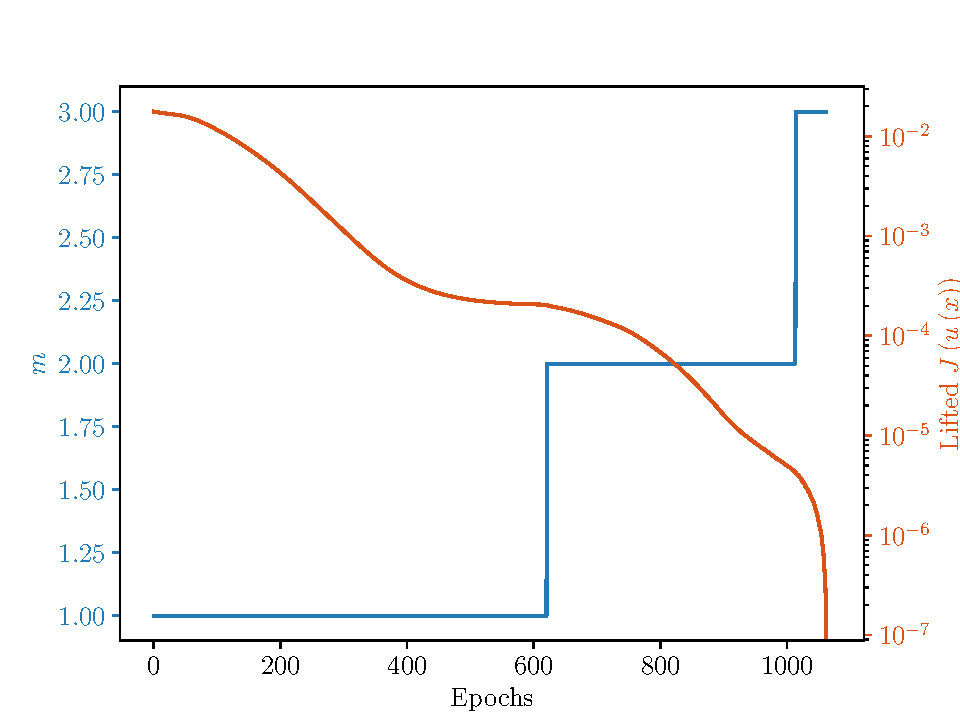
\includegraphics[width=\linewidth]{Figures/Loss_Modes.pdf}
		\caption{Loss decay and mode evolution}
	\end{subfigure}
	\begin{subfigure}[t]{0.5\linewidth}
		\centering
		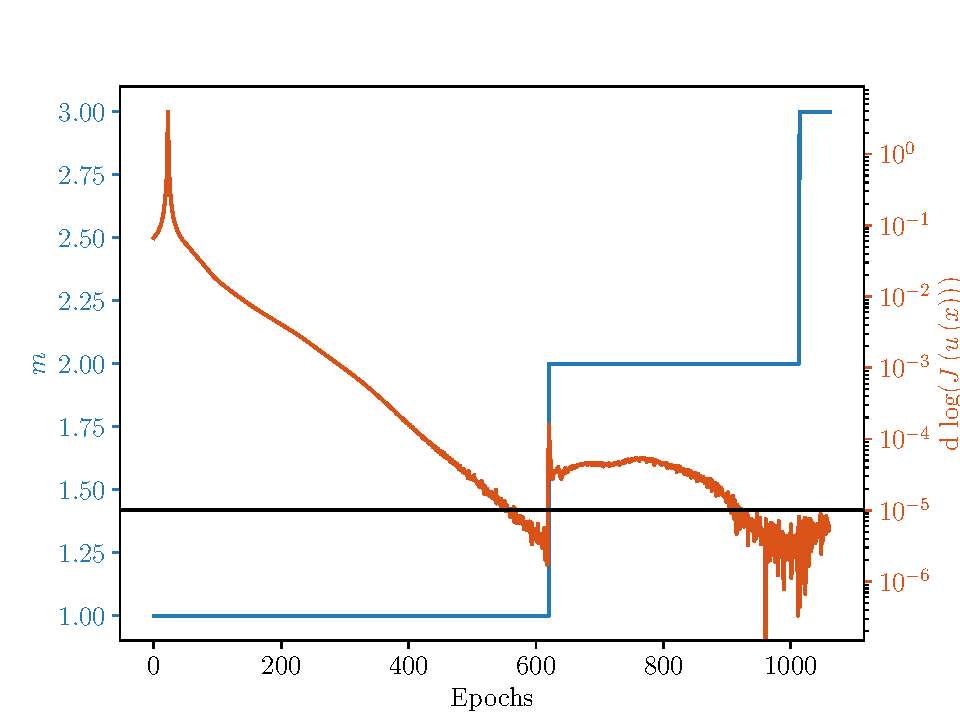
\includegraphics[width=\linewidth]{Figures/LossDecay_Modes.pdf}
		\caption{Loss logarithmic derivative and mode evolution}
	\end{subfigure}  
	\caption{Choice of the mode addition criterion}
	\label{fig:Criterion_mode}
\end{figure}

\begin{figure}
	\begin{subfigure}[t]{0.5\linewidth}
		\centering
		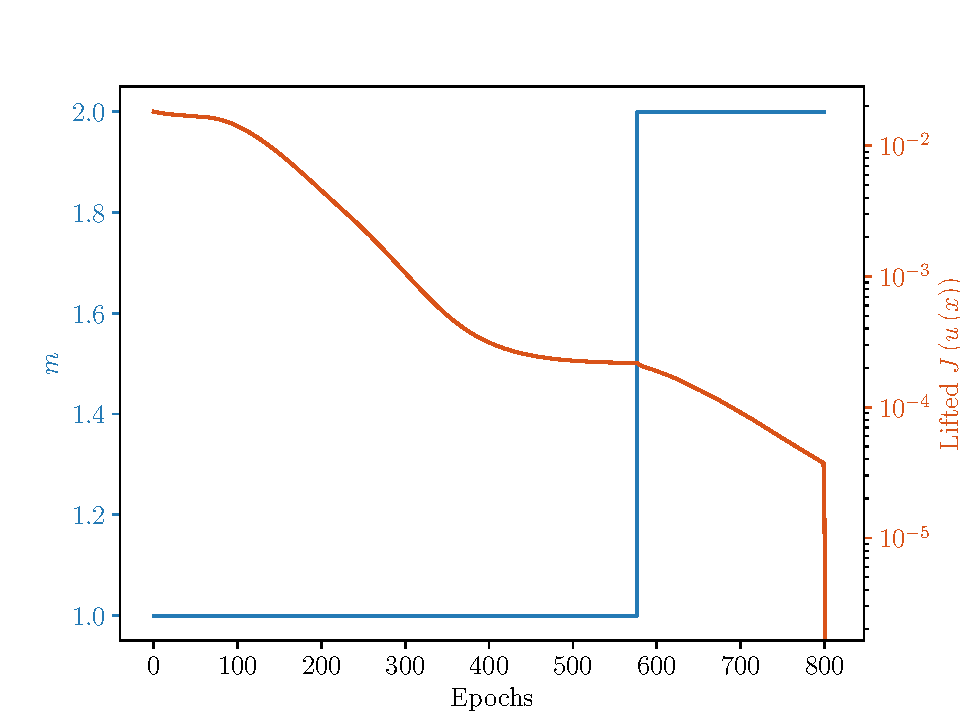
\includegraphics[width=\linewidth]{Figures/Loss_Modes_Bi_800.pdf}
		\caption{Loss decay and mode evolution}
	\end{subfigure}
	\begin{subfigure}[t]{0.5\linewidth}
		\centering
		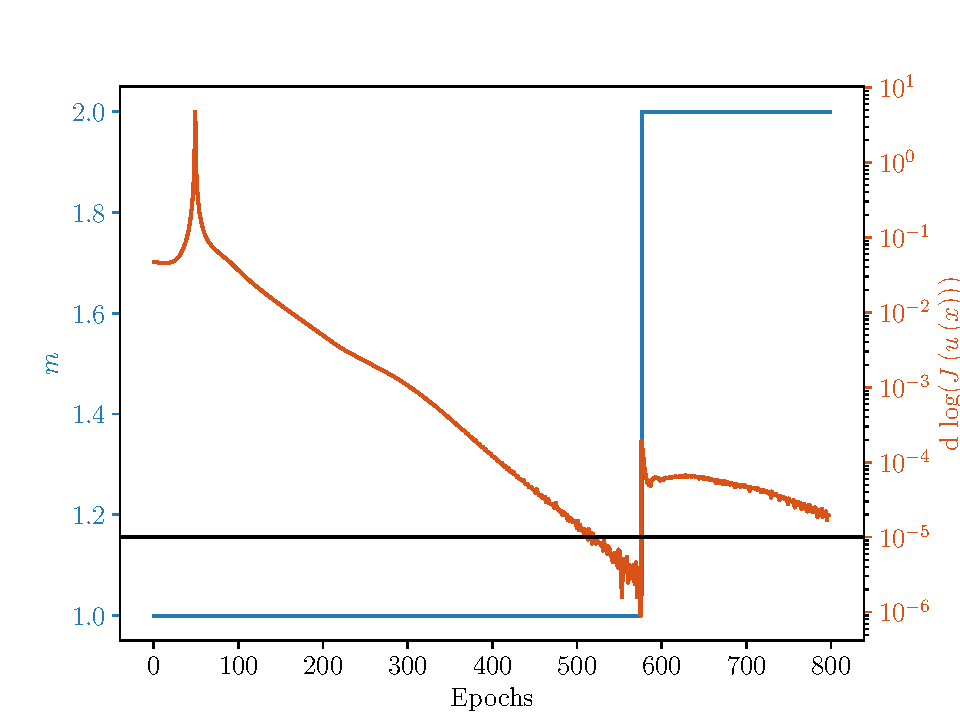
\includegraphics[width=\linewidth]{Figures/LossDecay_Modes_Bi_800.pdf}
		\caption{Loss logarithmic derivative and mode evolution}
	\end{subfigure}  
	\caption{Choice of the mode addition criterion for a different case}
	\label{fig:Criterion_mode2}
\end{figure}


\Rqs{Because we are looking at the lifted J, the very small decade crossing at the end are visible but do not appear in the derivation that is computed on the actual J and not the lifeted version (as the minimum is only known at the end of the minisation process)}{This is very visible when comparing error and lifted energy, see \cref{fig:Impact_lift}. We do not plot the energy but the energy error that tends to 0. But the derivative is computed on the energy... We need an \emph{a priori} error estimator that tends to 0 (that omit discretisation error for instance. Is is the case with the residual error given by the mixed formulation?)}

\begin{figure}
	\begin{subfigure}[t]{0.5\linewidth}
		\centering
		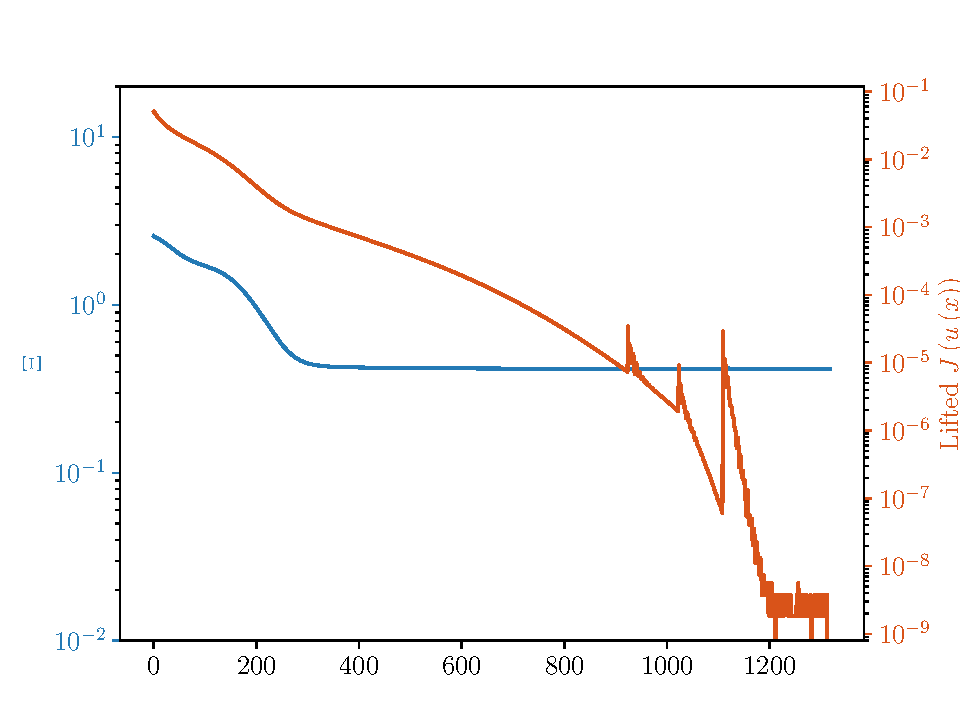
\includegraphics[width=\linewidth]{Figures/Loss_Error_Modes_Mono_1.pdf}
		\caption{Lifted loss and real L2 error}
	\end{subfigure}
	\begin{subfigure}[t]{0.5\linewidth}
		\centering
		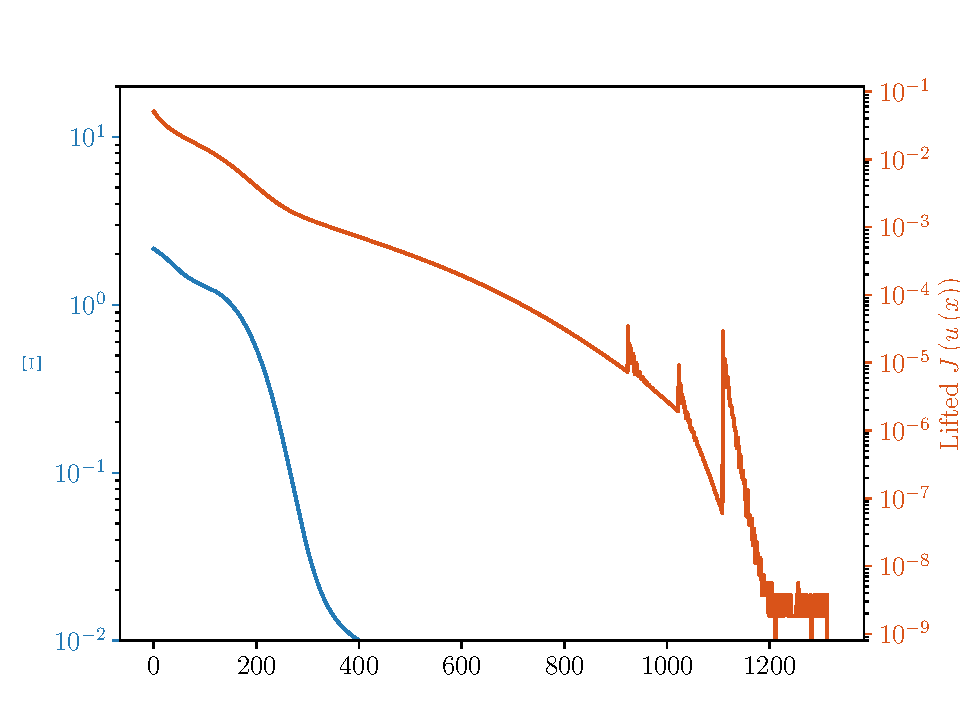
\includegraphics[width=\linewidth]{Figures/Loss_Error_Modes_Mono_2.pdf}
		\caption{Lifted loss and L2 error}
	\end{subfigure}  
	\caption{Impact of lifting}
	\label{fig:Impact_lift}
\end{figure}

It should be noted that here both the space and parametric modes are updated during the training which should theoretically be an improvement over the standard PGD method.


The final greedy algorithm is summarised in \cref{alg:GreedyPGD}.

\RestyleAlgo{ruled}

%% This is needed if you want to add comments in
%% your algorithm with \Comment
\SetKwComment{Comment}{/* }{ */}
\SetEndCharOfAlgoLine{}
\begin{algorithm}[hbtp!]
	\caption{Greedy algorithm}\label{alg:GreedyPGD}
	\textbf{Inputs: } \code{model}, 
	\code{optimizer},  
	\code{\arbitrary{max\_stgn}}, 
	\code{\arbitrary{threshold}}, 
	\code{\arbitrary{new\_mode\_threshold}}
	\textcolor{GreenLMS}{\Comment*[r]{Arbitrary values are highlighted in \arbitrary{red}}}
	
	
	\code{stgn = 0} 	\textcolor{GreenLMS}{\Comment*[r]{Number of consecutive stagnating epochs}}
	
	\code{loss\_decrease = 0 } 	\textcolor{GreenLMS}{\Comment*[r]{Arbitrary initial value}}
	
	\code{usefullness = 0} 	\textcolor{GreenLMS}{\Comment*[r]{Cumulative improving epochs since new mode}}
	
		\While(\textcolor{GreenLMS}{\Comment*[r]{\hspace{-5pt}Training loop \hspace{-6pt}}}){\emph{\code{epoch}} < \emph{\code{max\_epoch}}}{
		
    \If{\code{\emph{stgn}} > \code{\emph{\arbitrary{max\_stgn}}} \& \textbf{\emph{not}} \code{\emph{flag\_usefull}} }{
	Break\textcolor{GreenLMS}{\Comment*[r]{Break if previous mode did not stop stagnation}}
}


		$\mathcal{L} = J\left(\vect{u}\left((\textcolor{BleuLMS!70}{\vect{x}},\textcolor{LGreenLMS}{\left\{\mu^k\right\}}\right),\textcolor{BleuLMS!70}{\vect{x}},\mu\left(x\right)\right)$  \textcolor{GreenLMS}{\Comment*[r]{ Loss evaluation}}
		
		\eIf{\code{\emph{epoch>1}}}{
		\code{loss\_decrease} = $\frac{2\left(\text{\code{L\_old - L}}\right)}{\left|\text{\code{L\_old + L}}\right|}$ 	\textcolor{GreenLMS}{\Comment*[r]{Update loss decrease}}
		
		\eIf{$\left| \text{\code{\emph{loss\_decrease}}}\right| < \text{\code{\emph{\arbitrary{threshold}}}} $ }
		{\code{stgn} +=1  	\textcolor{GreenLMS}{\Comment*[r]{Increment stagnation}}
		}{
		\code{stgn}$=0$  	\textcolor{GreenLMS}{\Comment*[r]{Reset stagnation}}
		
		\If{\emph{\code{L}} $> 0$}{
			\code{usefullness} +=1 \textcolor{GreenLMS}{\Comment*[r]{ Check that loss decrease is more than a single spike}}
			
			\If{\emph{\code{usefullness>\arbitrary{10}} }}{
			\code{flag\_usefull = True} \textcolor{GreenLMS}{\Comment*[r]{ Previous mode flagged useful}}}  
		}
	}
		
		\code{L\_old} = L
		}{L\_old = L}
		
		
		\code{L.backward()}  \textcolor{GreenLMS}{\Comment*[r]{ Gradient of the loss}}
		\code{optimiser.step()}  \textcolor{GreenLMS}{\Comment*[r]{ Update the models}}
		
			\If{\code{\emph{stgn}} > \arbitrary{\code{\emph{new\_mode\_threshold}}}\& \code{\emph{flag\_usefull}} }{
			\code{model.AddMode()} 	\textcolor{GreenLMS}{\Comment*[r]{Add new mode}}
			
			\code{model.AddMode2Optimizer(optimizer)} 	\textcolor{GreenLMS}{\Comment*[r]{Add the new parameters to the optimizer}}
				
			\code{flag\_usefull = False} 
			
			
		}
	}
\end{algorithm}

\Rqs{The	\code{\arbitrary{max\_stgn}} and \code{\arbitrary{new\_mode\_threshold}} hyperparameters do not appear to change the behaviour be they chosen from $\simeq 5 - 100$ which is a good point. The real hyperparameter is the \code{\arbitrary{threshold}}.}{Could replace the first two by a hard threshold as classically done with a convergence criterion. Just have to be carefull with ``False'' imprvement due to new more when there is just a spike and not a substantive improvement.} 


\textbf{\textcolor{accentcolor}{Verification:}} check that it make sense that the usefulness has to get to 10 when stagnation max is only 5....

\textbf{\textcolor{accentcolor}{Answer:}} Yes it does, if it stops it means that its stagnating thus usefulness is not improving. 


\section{Literature review}

I cam across the work of \cite{lu_adaptive_2018} that seems very related to our work. It deals with 
\begin{itemize}
	\item Adaptative sampling in the parameter space
	\begin{itemize}
		\item But uses an \emph{a posteriori} refinement approach
		\item Needed to overcome uniform sampling in HD curse of dimensionality 
	\end{itemize}
	\item Geometry changes
	\begin{itemize}
		\item Using morphing techniques from introduced by \cite{galland_global_2011}
	\end{itemize}
	\item High-order PGD
	\begin{itemize}
		\item Only for snapshot compression
	\end{itemize}
\end{itemize}


\section{TODO}
\begin{itemize}
	\item Try the level-set function on coarse mesh parametrisation of the space clustering.
	\begin{itemize}
		\item First in 1D
		\item Then rely on the 2D developments to extend in 2D
	\end{itemize}
\end{itemize}
